\documentclass[12pt,onecolumn]{article}

\usepackage{xeCJK}
\usepackage{graphicx}

\setCJKmainfont{SimSun}
\setCJKsansfont{SimSun}
\setCJKmonofont{SimSun}
\setmainfont{Times New Roman}
\setsansfont{Times New Roman}
\setmonofont{Times New Roman}
\linespread{1.25}

\begin{document}
    \title{人工神经网络原理文献报告}
    \author{叶茂青}

    \maketitle
    用中文写一篇文献报告。文献报告要求突出但不限于几个要点:文章内容简述,主要贡献,个人理解与体会。并且自选多个角度,用图表形式对这些文章进行对比分析


    \section{Rich feature hierarchies for accurate object detection and semantic segmentation\cite{girshick2014rich}}
    提出了R-CNN这一网络架构,在传统的CNN架构上加入Region Proposal的结构,从而完成图像目标检测的任务。R-CNN完成图像目标检测的步骤如下:\par
    1. 使用Region proposals在原图像中取出大约2000个区域\par
    2. 使用一个CNN网络将提取出来的区域变为一个固定长度的特征\par 
    3. 使用SVM进行分类\\
    第一步Region proposals的方法采用Selective search,第二步使用预训练的Alexnet对输入为$227\times 227$的RGB图片抽取4096维的特征向量,最后采用SVM进行分类,并通过回归的方法修正Bounding box的误差。\\
    R-CNN的一些缺点:\par 
    1. Region proposals提取的区域会有重叠,送入CNN网络时会有很多重复计算\par 
    2. CNN网络需要固定尺寸的图片\par 
    3. 使用了SVM进行分类\par 

    \section{Spatial pyramid pooling in deep convolutional networks for visual recognition\cite{he2015spatial}}
    对于R-CNN中对图像进行裁剪后重新扩展到$227\times 227$作出了一点改进,提出了一种叫做Spatial pyramid pooling network的结构。\par 
    R-CNN中需要对裁剪的图像重新进行处理的原因是Alexnet最后为全连接层,需要保证输入的维数固定,Spatial pyramid pooling network通过将最后一层卷积层的输出,经过池化操作变为固定长度的特征向量,从而让网络可以接受任意大小的图片
    \begin{figure}[h]
        \centering
        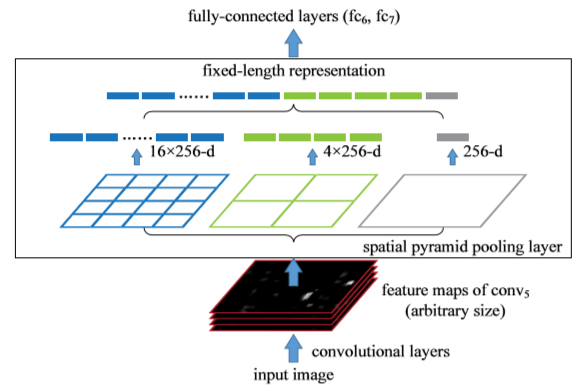
\includegraphics[width=\linewidth]{figure/spp.png}
        \caption{A network structure with a spatial pyramid pooling layer}
    \end{figure}
    如上图,Spatial pyramid pooling network通过将最后一层卷积层的输出分割成16份、4份、1份,再使用Max Pooling对每一份内的特征进行池化,最后拼接起来形成$21\times dimension$的特征向量作为全连接层的输入
    
    \section{Fast r-cnn\cite{girshick2015fast}}
    R-CNN需要把Region proposals选出的2000个区域都送入CNN进行计算,极大的降低了目标检测的效率,Fast R-CNN受Spatial pyramid pooling network的启发,在特征图上进行Region proposals。同时抛弃了R-CNN使用SVM进行分类的做法,直接用Softmax对分类进行预测,并引入multi-task loss。

    \section{Faster r-cnn: Towards real-time object detection with region proposal networks\cite{ren2015faster}}
    Fast R-CNN并没有完全做到end-to-end的训练,虽然只需要过一次CNN网络,但Region proposals部分依旧需要很长的时间,Faster R-CNN将Region proposals部分也融入到网络中,极大的提高了运算效率。相比之前的Selective search方法,Faster R-CNN引入了Region Proposal Networks来完成Region Proposal的任务。

    \section{You only look once: Unified, real-time object detection\cite{redmon2016you}}
    YOLO网络的基本想法:
    系统将输入图片分为$S\ast S$的网格单元。如果物体的中心落入某个格子,那么这个格子将会用来检测这个物体。
    每个网格单元会预测B个bounding box以及这些框的置信值。
    每个bounding box会有5个预测值:x,y,w,h和置信值confidence
    \begin{equation}
        confidence=Pr(Object)\ast IOU^{truth}_{pred}
    \end{equation}
    如果object落在一个网格单元里,$Pr(Object)$取1,否则取0。
    检测评价函数 intersection-over-union:
    \begin{equation}
        IOU=\frac{DetectionResult\cap GroundTruth}{DetectionResult\cup GroundTruth}
    \end{equation}
    每个网格单元也预测C个条件类概率,$Pr(Class_i|Object)$,在一个网格单元包含一个物体的前提下,它属于某个类的概率。我们只为每个网格单元预测一组类概率,而不考虑框B的数量。 
    在测试的时候,通过如下公式来给出对某一个box来说某一类的confidence score: 
    
    \begin{equation}
        Pr(Class_i|Object)\ast Pr(Object)\ast IOU^{truth}_{pred}=Pr(Class_i)\ast IOU^{truth}_{pred}
    \end{equation}

    然后设定阀值,过滤掉得分低的,对保留的boxes进行NMS处理,得到最终的检测结果。

    网络存在的问题:\par
    1. 由于输出层为全连接层,只能检测与训练图像相同分辨率的图像。\par
    2. 虽然每个格子可以预测 B 个 bounding box,但是最终只选择只选择 IOU 最高的 bounding box 作为物体检测输出,即每个格子最多只预测出一个物体。当物体占画面比例较小,如图像中包含畜群或鸟群时,每个格子包含多个物体,但却只能检测出其中一个。
    
    \section{Ssd: Single shot multibox detector\cite{liu2016ssd}}
    

    {\small
    \bibliographystyle{IEEEtran} 
    \bibliography{report.bib}
    }
\end{document}